\providecommand{\main}{..}
\documentclass[\main/notes.tex]{subfiles}

\begin{document}
	\ifSubfilesClassLoaded{\setcounter{chapter}{8}}{}
	\chapter{Programming Languages}
		\begin{definition}{Computer Language}
			A set of predefined words that are combined into a program according to predefined rules (\concept{syntax}).
		\end{definition}
		\section{Evolution}
			Computer languages have evolved from \concept{machine language} to \concept{high-level languages}.
			\subsection{Machine Languages -- First Generation}
				Each computer has its unique machine language -- a stream of $0$s and $1$s. The only language understood by the computer hardware. Computer hardware is made of electronic switches with two states: on and off.

				Disadvantages:
				\begin{itemize}
					\item Machine-dependent. The machine language of one computer is different from the machine language of another computer.
					\item Tedious to write programs in this language, and difficult to find errors.
				\end{itemize}
			\subsection{Assembly Languages}
				Replace binary code for instructions and addresses with symbols or mnemonics. First known as \concept{symbolic languages}, later called \concept{assembly languages}.

				An \concept{assembler} translates code from assembly language into machine language.

				Disadvantages:
				\begin{itemize}
					\item Programmers still have to concentrate on the hardware being used.
					\item Each machine instruction has to be individually coded, which makes using these languages tediuos.
				\end{itemize}
			\subsection{High-Level Languages}
				Portable to many different computers. The programmer can concentrate on the application, rather than the intricacies of the computer's organisation or hardware.

				Change the focus from the computer to the problem being solved.

				Must still be converted to machine language, called either \concept{interpretation} or \concept{compilation}.

		\section{Translation}
			Programs are normally written in a high-level language. To run the program, this code needs to be translated into machine language. The program that was written in the high level language is called the \concept{source program}. The translated program in machine language is called the \concept{object program}. To translate the program, either \concept{compilation} or \concept{interpretation} is used.

			\subsection{Compilation}
				A \concept{compiler} translates the whole source program into the object program.

			\subsection{Interpretation}
				An \concept{interpreter} translates each line of the source program into the corresponding line of the object program, and executes the line.

				\subsubsection{First Approach to Interpretation}
					Interpreted languages prior to Java (such as BASIC and APL) use this.

					Each line of the source program is translated into machine language, and then executed immediately. If there are errors, the process displays a message and terminates.

					Considered a slow process.
				\subsubsection{Second Approach to Interpretation}
					Introduced with Java.

					The translation of the source program is done in two steps: compilation and interpretation. A source program is first compiled to create \concept{bytecode}. This code is similar to machine language, but is not for any specific computer. This code is used by the \concept{Java Virtual Machine (JVM)}. The code is then run using a JVM emulator.
			\pagebreak

			\subsection{Translation Process}
				While the two methods above differ, they use the same translation process.
				\begin{center}
					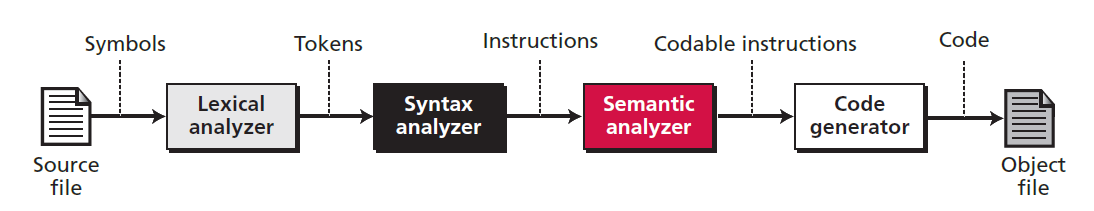
\includegraphics[width=0.9\textwidth]{\main/images/unit09/translation.png}
				\end{center}
				\begin{indentparagraph}
					\begin{description}
						\item[Lexical Analyzer] Reads the source code, symbol by symbol, and creates a list of \concept{tokens} in the source language. For example, the symbols \texttt{`w'`h'`i'`l'`e'} are grouped together as the token \texttt{while}.
						\item[Syntax Analyzer] Parses a set of tokens to find instructions. For example, the tokens \texttt{`x'`='`0'} would create the assignment statement \texttt{x=0}.
						\item[Semantic Analyzer] Checks the provided instructions to ensure there is no ambiguity. As programming languages are normally unambiguous, this state is either omitted in a \concept{translator}, or its duty is minimal.
						\item[Code Generator] Each unambiguous instruction is converted into a set of machine language instructions for the computer on which the program will run. 
					\end{description}
				\end{indentparagraph}

		\section{Programming Paradigms}
			\begin{definition}{Paradigm}
				A way in which a computer language looks at a problem to be solved. Four types: \concept{procedural (imperative)}, \concept{object-oriented}, \concept{functional}, and \concept{declarative}.
			\end{definition}
			\begin{center}
				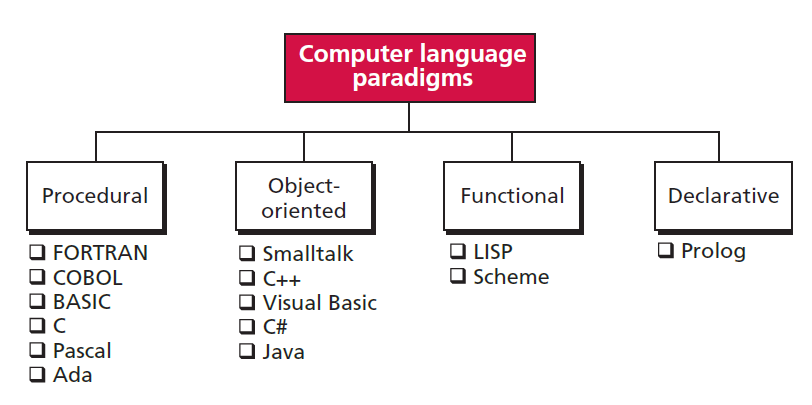
\includegraphics[width=0.9\textwidth]{\main/images/unit09/paradigms.png}
			\end{center}
			\subsection{Procedural (Imperative) Paradigm}
				A program is an \concept{active agent} that manipulates \concept{passive objects}.

				The passive objects (\concept{data} or \concept{data items}) are stored in memory, and a program manipulates them. To manipulate them, the program issues an action, called a \concept{procedure}.

				The program does not define the procedure -- it only triggers or calls the procedure.

				A program in this paradigm is made up of three parts:
				\begin{enumerate}[nosep]
					\item a part for object creation
					\item set of procedure calls
					\item set of code for each procedure
				\end{enumerate}
				\subsubsection{Some Procedural Languages}
					\begin{definition}{FORTRAN (FORmula TRANslation)}
						Designed by a group of IBM engineers under the supervision of Jack Backus. Commercially available in 1957. First high-level language.
						\begin{itemize}[nosep]
							\item High precision arithmetic
							\item Handle complex numbers
							\item Exponentiation computation ($a^{b}$)
						\end{itemize}
					\end{definition}
					\begin{definition}{COBOL (COmmon Business-Oriented Language)}
						Designed by a group of computer scientests under Grace Hopper of the US Navy. Focused on business needs.
						\begin{itemize}[nosep]
							\item Fast access to files and databases
							\item Fast uploading of files and databases
							\item Large amounts of generated reports
							\item User-friendly formatted output
						\end{itemize}
					\end{definition}
					\begin{definition}{Pascal}
						Designed by Niklaus Wirth in 1971 in Zurich, Switzerland. Named after Blaise Pascal. Popular language in academia.
					\end{definition}
					\begin{definition}{C}
						Developed in the early 1970s by Dennis Ritchie at Bell Laboratories. Originall intended for writing operating systems and system software -- most of UNIX is written in C.
						\begin{itemize}[nosep]
							\item Has all the high-level instructions a structured high-level programming language should have
							\item Also has low-level instructions that allow the programmer to access the hardware directly and quickly.
							\item Very efficient: the instructions are short.
						\end{itemize}
					\end{definition}
					\begin{definition}{Ada}
						Named after Augusta Ada Byron, duaghter of Lord Byron, and assistnt to Charles Babbage. Created by the US Department of Defence as a uniform language for all DoD contractors.
						\begin{itemize}[nosep]
							\item High-level instructions
							\item Instructions to allow real-time processing, which makes it suitable for process control.
							\item Parallel-processing capabilities.
						\end{itemize}
					\end{definition}
			\subsection{Object-Oriented Paradigm}
				Active objects instead of passive objects. The actions to be performed on the object are included in the object. Unlike the procedural paradigm, where procedures are separate entities, methods in OO belong to objects.
				\begin{indentparagraph}
					\begin{description}
						\item[Class] Group a set of methods that show how an object should react to external stimuli.
						\item[Methods] Similar to functions in procedural. Has a header, local variables, and statements.
						\item[Inheritance] When a more specific object or class gets functionality from a more general object or class.
						\item[Polymorphism] Define several operation with the same name that can do different things in related classes.
					\end{description}
				\end{indentparagraph}
				\subsubsection{Some Object-Oriented Languages}
					\begin{definition}{C++}
						Developed by Bjarne Stroustrup at Bell Laboratories as an improvement of the C~language. It uses \concept{classes} to define the general characteristics of similar objects and the operations that can be applied to them. Principles used in the design of C++ are:
						\begin{itemize}[nosep]
							\item encapsulation
							\item inheritance
							\item polymorphism
						\end{itemize}
					\end{definition}
					\begin{definition}{Java}
						Developed at Sun Microsystems, Inc. Based on C and C++, but removed some features from C++ to make the language more robust.

						The language is entirely object-oriented, unlike C++. A program can be either an application or an applet. An applet is embedded HTML, stored on a server and run by a browser.

						A program is a collection of classes and instances of those classes. The \concept{class library} is a collection of classes, and new classes can be built based on those in the library.

						Execution of a program is unique -- create a class and pass it to the interpreter, and the interpreter calls the class methods. Java supports \concept{multithreading.}, whereas C++ only supports single threading.
							\begin{indentparagraph}
								\begin{description}
									\item[Thread] A sequence of actions executed one after another.
								\end{description}
							\end{indentparagraph}
					\end{definition}
			\subsection{Functional Paradigm}
				A program is considered a mathematical function. A function can be considered a black box that maps a list of inputs to a list of outputs.

				A functional language does the following:
				\kern-\parskip\begin{itemize}[nosep]
					\item Predefine a set of primitive (atomic) functions that can be used by any programmer
					\item Allow a programmer to combine primitive functions to create new functions
				\end{itemize}

				Advantages over procedural languages:
				\begin{itemize}[nosep]
					\item Encourages modular programming
					\item Allows programmers to make new functions out of existing ones
				\end{itemize}

				\subsubsection{Some Functional Languages}
					\begin{definition}{LISP (LISt Programming)}
						Designed by a team of researches at MIT in the early 1960s. A list-processing language in which everything is considered a list.
					\end{definition}
					\begin{definition}{Scheme}
						A standardized version of LISP developed by MIT in the early 1970s.

						Defines a set of primitive functions that solve problems. The function name and the list of inputs to the function are enclosed in parentheses. 
					\end{definition}
				\subsection{Declarative Paradigm}
					Uses the principle of logical reasoning to answer queries. Based on formal logic and \concept{first-order predicate calculus}. Based on deduction.

					A program written in these languages is specfic to a particular domain, as collecting all the facts into a program makes it huge.

					Limited so far to fields such as artificial intelligence.
					\subsubsection{Some Declarative Languages}
						\begin{definition}{Prolog (PROgramming in LOGic)}
							Developed by A. Colmerauer in France in 1972. A program is made up of facts and rules.
						\end{definition}
		\rulechapterend
\end{document}